\documentclass[12pt]{report}

\usepackage[left=0.5in, right=0.5in, top=0.5in, bottom=0.5in]{geometry}
\setlength\parindent{0pt}
\usepackage{epsfig,graphics,amsmath,color,multicol,enumerate,tabularx,pbox,bm}


\setlength\parindent{0pt}

\usepackage{graphicx, amsmath,anonchap,tabularx,multicol,enumitem}
\usepackage{lscape,mdwlist}

\usepackage{enumitem}
\setlist{noitemsep}
\setlist{nolistsep}

\newenvironment{boxe}
    {\begin{center}
    \begin{tabular}{|p{0.9\textwidth}|}
    \hline\\
    }
    { 
    \\\hline
    \end{tabular} 
    \end{center}
    }

\begin{document}

%%INTEGRALS - FToC%%

\pagenumbering{gobble}

\begin{tabular*}{\textwidth}{@{\extracolsep{\fill}}l l}
\textbf{FUNdamental Theorem of Calculus}  & Funny Name: \rule{6cm}{0.5pt}\\

\hline\hline
\end{tabular*} \\
\smallskip

\begin{boxe}
    {\bf Fundamental Theorem of Calculus}:

If $f$ is continuous on $[a,b]$ and $f(t)=F\,'(t)$, then 
$$\int_a^bf(t)\,dt=\int_a^bF'(t)\,dt=F(b)-F(a)$$
\end{boxe}


\begin{enumerate}[start=2]
% removed this activity
\iffalse
\item The concentration of a medication in the plasma changes at a rate of $h(t)$ mg/ml per hour, $t$ hours after the delivery of the drug.

(a) Explain the meaning of the statement $h\left(1\right)=50$. Include units. \vskip .75in

(b) If $H\ '(t)=h(t)$, what are the units on $H(t)$?\vskip .75in

(c) There are $250\ \frac{mg}{ml}$of the medication present at time $t=0$ and $\int_{0}^{3}h\left(t\right)dt=480$. What is the plasma concentration of the medication present three hours after the drug is administered, $H\left(3\right)$? Do the units make sense? \vskip .75in
\fi
\item Water is leaking out of a tank at a rate of $r\left(t\right)$ gallons/hour, where $t\ $is measured in hours. Write a definite integral that expresses the total amount of water that leaks out in the first three hours. 
\vskip .75in
\begin{multicols}{2}
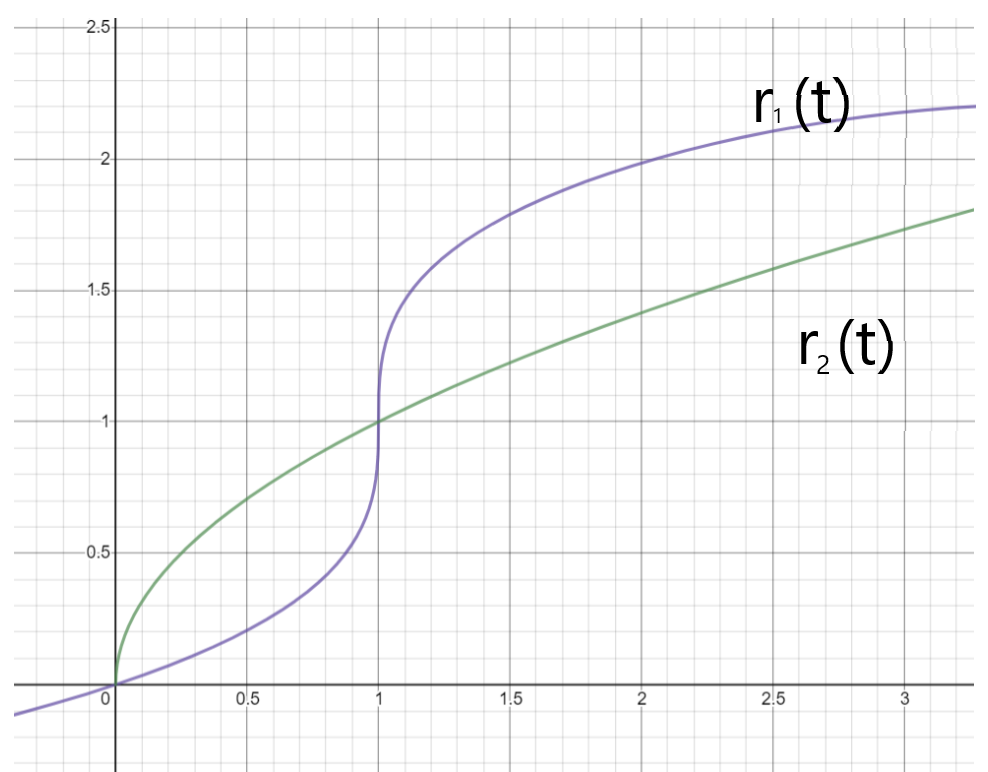
\includegraphics[width=.45\textwidth]{2rates.png}
Suppose the purple line represents $r_{1}(t)$ for tank 1 and the green line represents $r_{2}(t)$ for tank 2. 

(1) Which tank leaks more water in the first hour? Explain in terms of definite integrals and area. \vskip 1.5in

(2) Which tank leaks more water after 3 hours? Explain.



\end{multicols}

\item Biological activity in water is reflected in the rate at which carbon dioxide, CO$_{2}$, is added or removed. Plants take CO$_{2}$ out of the water during the day for photosynthesis and put CO$_{2}$ into the water at night. Animals put CO$_{2}$ into the water all the time as they breathe. The graph shows the rate of change of the CO$_{2}$ level in a pond. At dawn(t=0), there were 2.600 mmol of CO$_{2}$ per liter of water.

\begin{multicols}{2}
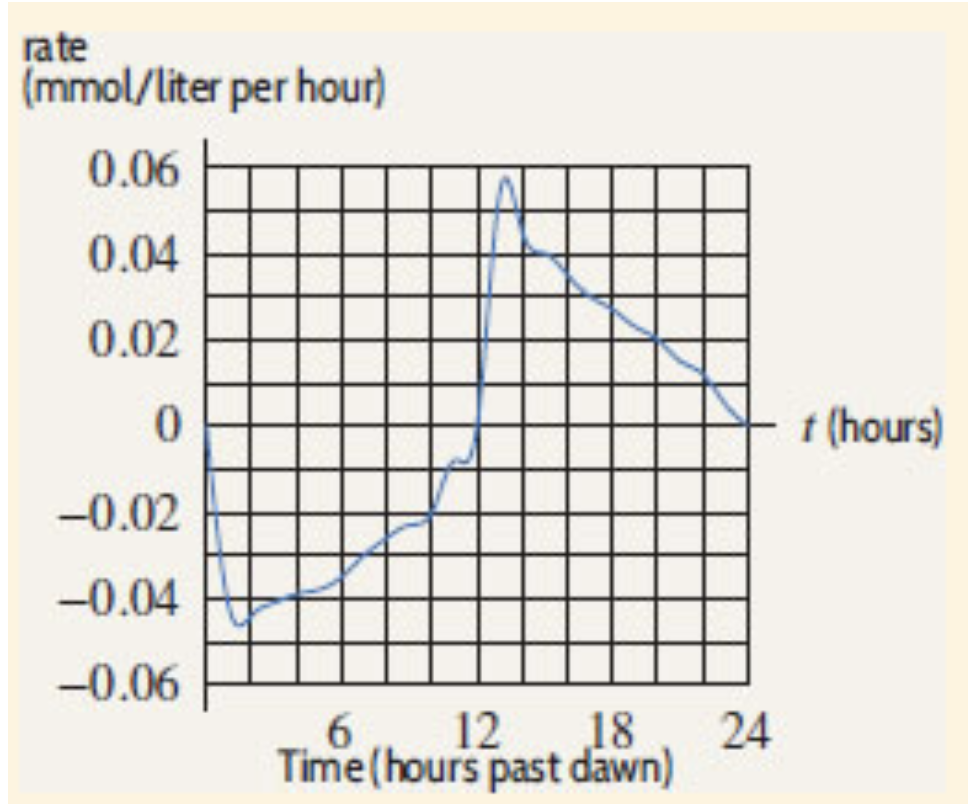
\includegraphics[scale=0.5]{biol.png}

(1) At what time was the CO$_{2}$ level lowest between 0 and 24? When was it highest?
\vskip 1in
(2) We know the initial amount of $CO_{2}$ at $t=0$ is 2.600 mmol/liter (i.e. $F\left(0\right)=2.6$). If a computer tells us that $\int_{0}^{12}f\left(t\right)dt=-0.328$, what is the $CO_{2}$ level 12 hours after dawn? (i.e. how many mmol/liter of $CO_{2}$ are present at $t=12$)
\end{multicols}
\vskip .75in
\item Let $C(n)$ be a city's cost, in millions of dollars, for plowing the roads when $n$ inches of snow have fallen. Let $c\left(n\right)=C\ '\left(n\right)$. Suppose you know the following:
\begin{multicols}{2}
$\;\;\;\;\;\;\;\int_{0}^{15}c\left(n\right)dn=7.5$

$\;\;\;\;\;\;\;c\left(15\right)=0.7$

$\;\;\;\;\;\;\;c\left(24\right)=0.4$

$C\left(15\right)=8$

$C\left(24\right)=13$\\
\end{multicols}



Answer the following questions:

(1) Evaluate $\int_{15}^{24}c\left(n\right)dn$\\ \vskip .5in

(2) Describe what (1) means (the integral and the answer) in a sentence using context of the problem.\\ \vskip .5in

(3) What is the value of $C\left(0\right),$ including units?\\\\\\

\item $G\left(x\right)=\ln\left(x\right)$. What is the total change of $G$ from $x=1$ to $x=e^5$?\vskip .5in
 
If $G\left(x\right)=\ln\left(x\right)$. Find $g(x)$ where $G'(x)=g(x)$.\vskip .5in
 
Write the definite integral $\int_{a}^{b}g\left(x\right)dx$ between $a=1,\ b=5$. Evaluate your integral exactly.\\\\\\\\\\

\item Evaluate the following definite integrals exactly using the FUNdamental Theorem of Calculus (Hint: find $F\left(x\right)$ by asking ``what function has $f\left(x\right)$ as its derivative?'' Or you can use geometry to come up with your answer.)

\begin{enumerate}[parsep=.7in]
\item $\displaystyle \int_{0}^{10}5\ dx$ 

\item $\displaystyle \int_{0}^{7}6x\ dx$

\item $\displaystyle \int_{-2}^{4}\left(\frac{1}{5}x-1\right)dx$ % this is HW problem fall 2022

\end{enumerate}
\end{enumerate}
\end{document}